%%% Econ761: IO Theory
%%% Fall 2021
%%% Danny Edgel
%%%
% Due on Canvas Tuesday, November 2nd, 11:59pm Central Time
%%%

%%%
%							PREAMBLE
%%%

\documentclass{article}

%%% declare packages
\usepackage{amsmath}
\usepackage{amssymb}
\usepackage{array}
\usepackage{bm}
\usepackage{bbm}
\usepackage{changepage}
\usepackage{centernot}
\usepackage{graphicx}
\usepackage{xcolor}
\usepackage[shortlabels]{enumitem}
\usepackage{fancyhdr}
	\fancyhf{} % sets both header and footer to nothing
	\renewcommand{\headrulewidth}{0pt}
    \rfoot{Edgel, \thepage}
    \pagestyle{fancy}
	
%%% define shortcuts for set notation
\newcommand{\Z}{\mathbb{Z}}
\newcommand{\R}{\mathbb{R}}
\newcommand{\Q}{\mathbb{Q}}
\newcommand{\lmt}{\underset{x\rightarrow\infty}{\text{lim }}}
\newcommand{\neglmt}{\underset{x\rightarrow-\infty}{\text{lim }}}
\newcommand{\zerolmt}{\underset{x\rightarrow 0}{\text{lim }}}
\newcommand{\loge}[1]{\text{log}\left(#1\right)}
\newcommand{\usmax}[1]{\underset{#1}{\text{max }}}
\newcommand{\usmin}[1]{\underset{#1}{\text{min }}}
\newcommand{\Mt}{M_{t+1}^t}
\newcommand{\vhat}{\hat{v}}
\newcommand{\olp}{\overline{p}}
\renewcommand{\L}{\mathcal{L}}
\newcommand{\olq}{\overline{q}}
\newcommand{\zinf}{_{t=0}^\infty}
\newcommand{\aneg}{A^{-1}}
\newcommand{\sneg}{s^{-1}}
\newcommand{\olk}{\overline{k}}
\newcommand{\one}[1]{\mathbbm{1}\left\{#1\right\}}
\newcommand{\olc}{\overline{c}}
\newcommand{\olr}{\overline{r}}
\newcommand{\olpi}{\overline{\pi}}
\newcommand{\Aneg}{A^{-1}}
\renewcommand{\sneg}{s^{-1}}
\newcommand{\dc}[1]{\Delta c_{#1}}
\newcommand{\N}{\mathcal{N}}
\newcommand{\suminf}{\sum_{t=0}^\infty}
\newcommand{\sumn}{\sum_{i=1}^{n}}
\newcommand{\sumnk}{\sum_{i=1}^{N_k}}
\newcommand{\red}[1]{{\color{red}#1}}
\newcommand{\Tau}{\mathrm{T}}
\newcommand{\phat}{\hat{p}}
\newcommand{\bhat}{\hat{\beta}}
\newcommand{\ahat}{\hat{\alpha}}
\newcommand{\qs}{q^*}
\newcommand{\pl}{\partial}

\newcommand{\E}[1]{\mathbb{E}\left[#1\right]} % expected value
\newcommand{\Et}[1]{\mathbb{E}_t\left[#1\right]}

%%% define column vector command (from Michael Nattinger)
\newcount\colveccount
\newcommand*\colvec[1]{
        \global\colveccount#1
        \begin{pmatrix}
        \colvecnext
}
\def\colvecnext#1{
        #1
        \global\advance\colveccount-1
        \ifnum\colveccount>0
                \\
                \expandafter\colvecnext
        \else
                \end{pmatrix}
        \fi
}

%%% define function for drawing matrix augmentation lines
\newcommand\aug{\fboxsep=-\fboxrule\!\!\!\fbox{\strut}\!\!\!}

\makeatletter
\let\amsmath@bigm\bigm

\renewcommand{\bigm}[1]{%
  \ifcsname fenced@\string#1\endcsname
    \expandafter\@firstoftwo
  \else
    \expandafter\@secondoftwo
  \fi
  {\expandafter\amsmath@bigm\csname fenced@\string#1\endcsname}%
  {\amsmath@bigm#1}%
}


%________________________________________________________________%

\begin{document}

\title{	Problem Set \#3 }
\author{ 	Danny Edgel 					        	      \\ 
			Econ 761: Industrial Organization Theory	\\
			Fall 2021						                      \\
		}
\maketitle\thispagestyle{empty}


%%%________________________________________________________________%%%

\section{Nevo's Code}

\subsection*{Multinomial Logit}
The table below displays the estimates for the coefficient on price, $\alpha$, for each specification. It is generated by the attached code, edgel\_ps3.tex. Note that there are fewer observations than are in the data provided; this is due to the specification requiring an ``outside option'', for which I chose the first brand.
\begin{center}
        \begin{tabular}{r|cccc}
 & (1) & (2) & (3) & (4) \\ 
& OLS & OLS & IV & IV \\\hline 
$\alpha$ & -30.036 & -27.988  & -30.071  & -39.603 \\ 
& (0.216) & (0.918) & (0.216) & (0.743) \\ 
 &&&& \\ 
FE? & & X & & X \\ 
 &&&& \\ 
$R^2$ & -0.32 & 0.46 & -0.32 & 0.39 \\
N & 2256 & 2256 & 2256 & 2256 \\\hline 
\end{tabular}
\end{center}
I calculate the multi-product Bertrand-Nash markups, $\mu\in\R^{j\times t}$, as\[ 
        \mu = \Omega^{-1}s
        \mu_j = \frac{s_j}{\pl s_j / \pl\delta_j} = \frac{1}{(1-s_j)\alpha}
\]
Where ${s}$ is the vector of market shares for each brand in each quarter and city, and \begin{align*}
        \Omega = \Omega^*\odot H,\quad &H_{ij} = \frac{\pl s_j}{p_j}    \\
        &\Omega^*_{ij} =  \begin{cases} 1, & i\text{ and }j\text{ are owned by the same firm} \\ 0, &\text{otherwise} \end{cases}
\end{align*}
Thus, by decomposing price into marginal cost and markup, we can also back out firm $j$'s marginal cost, $c_j$, and calculate its margin, $m_j$: \[
        c_j = p_j - \mu_j,\quad m_j = \frac{p_j}{c_j} - 1
\]
Using each $\hat{\alpha}$ from the table above, the mean, median, and standard deviation of markups, margins, and implied marginal costs under each specification are given in the table below.
\begin{center}
        \begin{tabular}{r|cccc}
 & (1) & (2) & (3) & (4) \\\hline &&&& \\ 
\E{\mu_{jt}} & -0.098 & 0.005  & -0.025  & 0.007 \\ 
Var(\mu_{jt})& 0.033 & 0.000 & 0.002 & 0.000 \\
 &&&&\\ 
\E{c_{jt}} & 0.224 & 0.121  & 0.150  & 0.119 \\ 
Var(c_{jt})& 0.035 & 0.001 & 0.003 & 0.001 \\
 &&&&\\ 
\E{m_{jt}} & -0.299 & 0.044  & -0.127  & 0.075 \\ 
Var(m_{jt})& 0.054 & 0.009 & 0.020 & 0.033 \\
&&&&\\\hline 
\end{tabular}
\end{center}
With the pre-merger marginal cost and $\alpha$ estimates, we have $J\times C\times T$ equations and as many unknowns for the post-merger equilibrium using the Bertrand-Nash equilibrium conditions. Following Nevo (2000), the new price vector, $p$, solves \[ 
        p = \hat{mc} + \Omega_{m}^{-1}s(p)
\]
Where $\Omega_m$ is the post-merger $\Omega$ matrix. 
However, the solution does not have a closed form. Instead, we can simulate any merger by:
\begin{enumerate}
        \item Changing $\Omega^*$ according to the new ownership structure
        \item Using the pre-merger price vector, $p_0$, and its associated shares, $s_0$, as an initial guess for the equilibirum
        \item Updating prices using the equilibrium condition and estimated values $\hat{mc}$ and $\ahat$ with the post-merger ownership matrix, $\Omega^*_{post}$ to calculate ${p_1 = \hat{mc} + \Omega^{-1}s_0}$
        \item If $||p_1-p_0||$ is greater than some negligible tolerance value, updating shares and $\Omega$ according to $p_1$ and repeating until convergence to $p$'s fixed point
\end{enumerate}
The results for post-merger prices and shares are displayed in the table below.
\begin{center}
        \begin{tabular}{r|ccccccccc}
 & \multicolumn{4}{c}{Post-Nabisco} & & \multicolumn{4}{c}{GM-Quaker} \\ 
 & (1) & (2) & (3) & (4) && (1) & (2) & (3) & (4) \\\hline&&&&&&&&&\\ 
$\E{p}$ & 0.124 & 0.124  & 0.124  & 0.124&& 0.125 & 0.125  & 0.125  & 0.125 \\ 
Med($p$)& 0.122 & 0.122 & 0.122 & 0.122&& 0.123 & 0.123  & 0.123  & 0.123 \\ 
Var($p$)& 0.001 & 0.001 & 0.001 & 0.001&& 0.001 & 0.001  & 0.001  & 0.001 \\
 &&&&&&&&&\\ 
$\E{s}$ & 0.029 & 0.020  & 0.020  & 0.017&& 0.030 & 0.020  & 0.020  & 0.016 \\ 
Med($s$)& 0.013 & 0.011 & 0.011 & 0.009&& 0.016 & 0.011  & 0.011  & 0.009 \\ 
Var($s$)& 0.002 & 0.001 & 0.001 & 0.001&& 0.002 & 0.001  & 0.001  & 0.001 \\
 &&&&&&&&&\\ 
\end{tabular}
\end{center}
The problem with this analysis is that we assume that any heterogeneity in consumer preferences and price sensitivity is independent, identically distributed, and orthogonal to utility. These assumptions are dibious and likely result in unrealistic estimations of counter-factuals. We can remedy these issues with a random coefficients model that interacts consumer demographics with prices and product characteristics, which will capture the observable heterogeneity in consumer preferences and price sensitivity.

\subsection*{Random Coefficients}
The results of the random coffecients estimation are provided below and are consistent with those in results.txt.
\begin{center}  
        \begin{tabular}{r|cccccc}
 & Mean & $\Sigma$ & Income & Income$^2$ & Age & $\one{\text{Child}}$ \\\hline &&&&&&\\ 
Constant   & -2.314 & 0.377  & 3.089  & 0.000 & 1.186 & 0.000\\ 
 & (0.246) & (0.122)  & (1.007)  & (0.000) & (1.010) &(0.000) \\ 
Price & -32.430 & 1.848  & 16.598  & -0.659 & 0.000 & 11.624 \\ 
 & (4.826) & (0.978)  & (104.545)  & (5.457) & (0.000) &(5.137) \\ 
Sugar & 0.117 & -0.003  & -0.193  & 0.000 & 0.030 & 0.000 \\ 
 & (0.246) & (0.012)  & (0.040)  & (0.000) & (0.034) &(0.000) \\ 
Mushy & 0.271 & 0.081  & 1.468  & 0.000 & -1.514 & 0.000 \\ 
 & (0.012) & (0.198)  & (0.676)  & (0.000) & (1.095) &(0.000) \\ 
 &&&&&& \\ 
\multicolumn{7}{l}{GMM objective: 14.998} \\ 
\multicolumn{7}{l}{MD $R^2$: 0.395} \\ 
\multicolumn{7}{l}{MD weighted $R^2$: 0.077} \\\hline 
\end{tabular}
\end{center}
Using this demand specification, the new estimates for markups and marginal costs are summarized below. 
\begin{center}  
        \begin{tabular}{r|ccc}
 & Mean & Median & Variance \\\hline &&& \\ 
 Markups   & -0.043 & -0.042 & 0.000 \\ 
 MC        & 0.168 & 0.166 & 0.001 \\ 
 &&& \\\hline 
\end{tabular}
\end{center}
I do not have the time to repeat the merger simulations with these results.

%%%________________________________________________________________%%%

\section{pyBLP}

The screenshot below displays the random coefficients estimates using the pyBLP package.
\begin{center}
        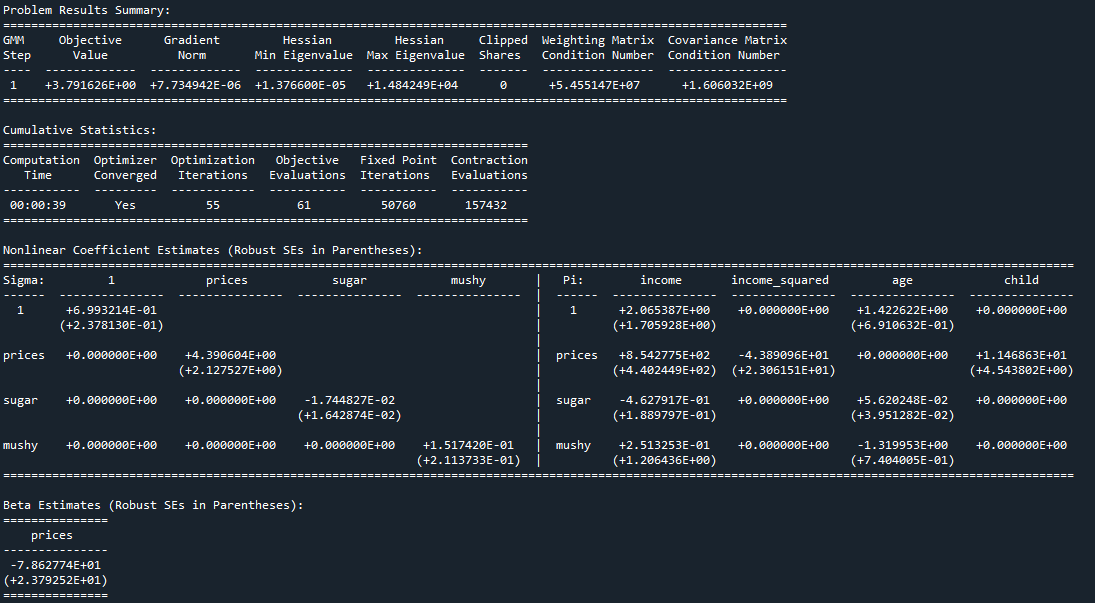
\includegraphics[scale = .5]{figure1.png}
\end{center}
The markup and marginal cost estimates are displayed below, confirming that my estimates from the Matlab code are far off.
\begin{center}
        \begin{tabular}{r|ccc}
 & Mean & Median & Variance \\\hline &&& \\ 
 Markups   & 0.372 & 0.345 & 0.018 \\ 
 MC        & 0.081 & 0.080 & 0.001 \\ 
 &&& \\\hline 
\end{tabular}
\end{center}
Notably, these markup estimates are far higher than those derived from the logit regression. Unfortunately, I do not have the time to repeat the merger simulations with these results.

\end{document}






